\documentclass{beamer}
\usetheme{Boadilla}

\usepackage{graphicx}
\usepackage{tikz}

\usetikzlibrary{positioning, arrows.meta, calc, fit, shapes, decorations.pathreplacing, backgrounds}
\tikzstyle{fancytitle} =[fill=white, text=black, draw]

\definecolor{colorThree}{HTML}{CC6633}
\definecolor{tikzDarkGreen}{HTML}{006622}
\definecolor{tikzBack}{HTML}{e0e0eb}

\setbeamertemplate{note page}[plain]
\setbeameroption{show notes}

\title[Reconstructing MetiTarski Proofs in Isabelle]{Reconstructing MetiTarski Proofs in Isabelle/HOL}
\subtitle {End-of-internship Presentation}
\author{Cristina Matache}
\institute[]{
\includegraphics[scale=0.45]{ai_logo_title}}
\date{September 22, 2017}

%Remove the navigation buttons
\setbeamertemplate{navigation symbols}{}

\begin{document}

\begin{frame}
\titlepage
\end{frame}

\begin{frame}
\frametitle{Outline}
\tableofcontents
\end{frame}

\section{MetiTarski}

\begin{frame}
\frametitle{MetiTarski}
\begin{itemize}
\item Automatic theorem prover (ATP)
\item Proves universally quantified inequalites involving:
	\begin{itemize}
	\item polynomials
	\item real-valued special functions: $log$, $exp$, $sin$, $cos$, $sqrt$ etc.
	\end{itemize}
\item Using:
	\begin{itemize}
	\item resolution
	\item a decision procedure for the theory of real closed fields (RCF)
	\end{itemize}
\item The special functions are \textit{approximated} by polynomials. So Metitarski is incomplete. (Without the approximations, the problem is undecidable.)			
\end{itemize}
\end{frame}

\begin{frame}
\frametitle{Motivation}

\begin{itemize}
\item Long-term goal: use MetiTarski inside Imandra to solve geometric problems
	\note[item]{These can be encoded as inequalities that MT understands.}
	
\item Why translate MetiTarski proofs to Isabelle proofs?
	\note[item]{If we want to use MT to verify things, we need very high confidence in its proofs.}
\begin{itemize}
\item No formal guarantee that the MetiTarski proofs are correct.
	\note[item]{MetiTarski was coded in Standard ML and there is no guarantee the code or the output is correct. Although it has of course been tested.}
\item Isabelle is more trustworthy than MetiTarski
\item If proof reconstruction is available, MetiTarski can be included as an automated tool in Isabelle
\end{itemize}
\end{itemize}
\end{frame}

\begin{frame}
\frametitle{The Problem}

\begin{minipage}{0.3\linewidth}
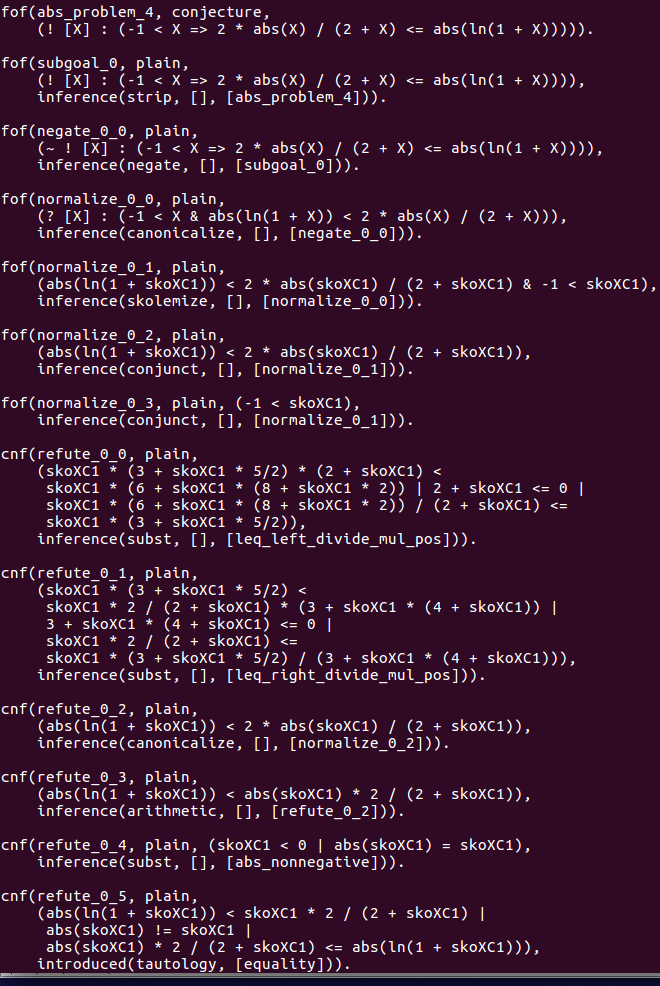
\includegraphics[scale=0.2]{MT_proof}
\end{minipage}
\hfill
\begin{minipage}{0.57\linewidth}
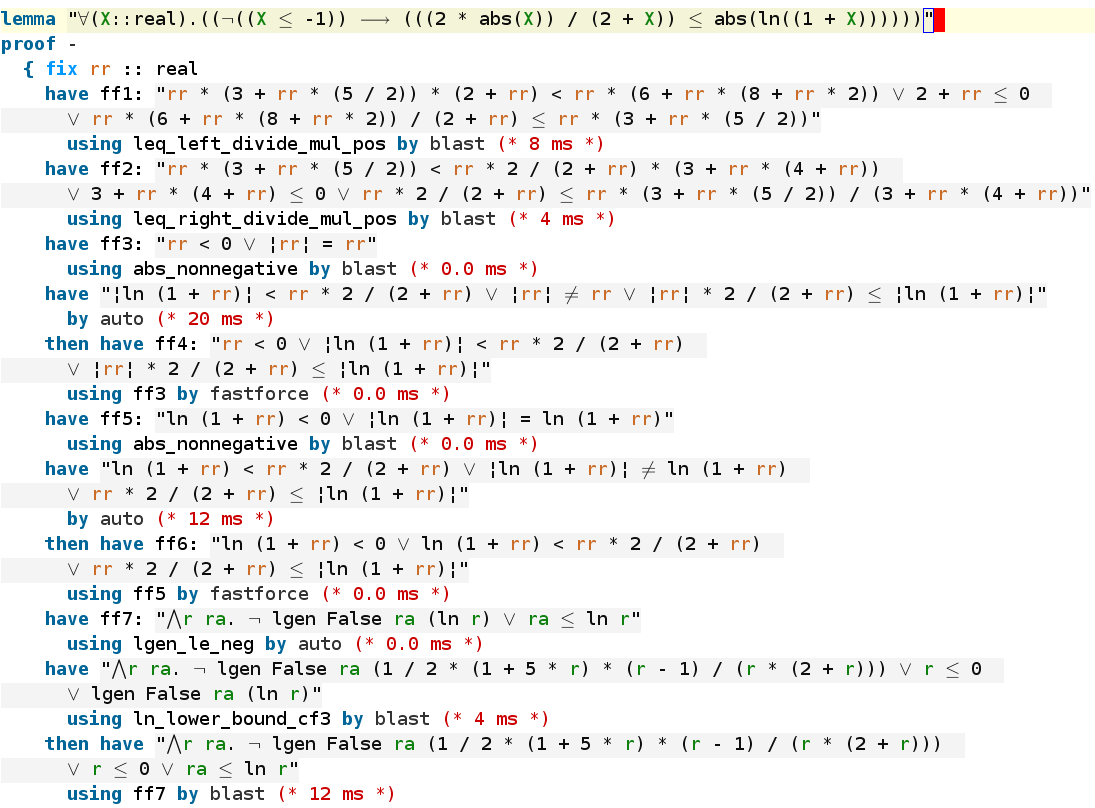
\includegraphics[scale=0.18]{isabelle_proof}
\end{minipage}

%Side by side picture of an MT and Isabelle proofs
	\note[item]{We need to turn this MT proof into an Isabelle proof. You probably can't read this because the proofs look horrible, and that's exactly the point. You want to be able to do this translation automatically. Roughly what happens is that every step in the MT proof corresponds to a "have" in Isabelle and a proof method.}
	\note[item]{In Isabelle, the way you do proofs is you can specify intermmediate steps, prove them, and then use them later to prove your conclusion. To prove things you need to specify a proof method, there are maybe 10-15 that are commonly used. And sometimes you have to give Isabelle hints about what lemmas to use.}
\end{frame}

\section{Sledgehammer}

\begin{frame}
\frametitle{Sledgehammer}

\begin{itemize}
\setlength\itemsep{1em}
\item Automatic proof tool in Isabelle.
	\note[item] {It turns out there is a tool in Isabelle that does something similar. Isabelle is an \textit{interactive} theorem prover so it normally requires a lot of user input to do a proof, the user has to specify what steps should be taken. Sledgehammer aims to improve automation.}
	
	\note[item] {Sledgehammer tries to automatically find a proof for the given lemma without any user input. What it does is it calls a bunch of ATPs and tries to translate their proofs into Isabelle proofs. Which is exactly what I need to do.}

\item Sledgehammer operation:
\end{itemize}

	
\begin{figure}	
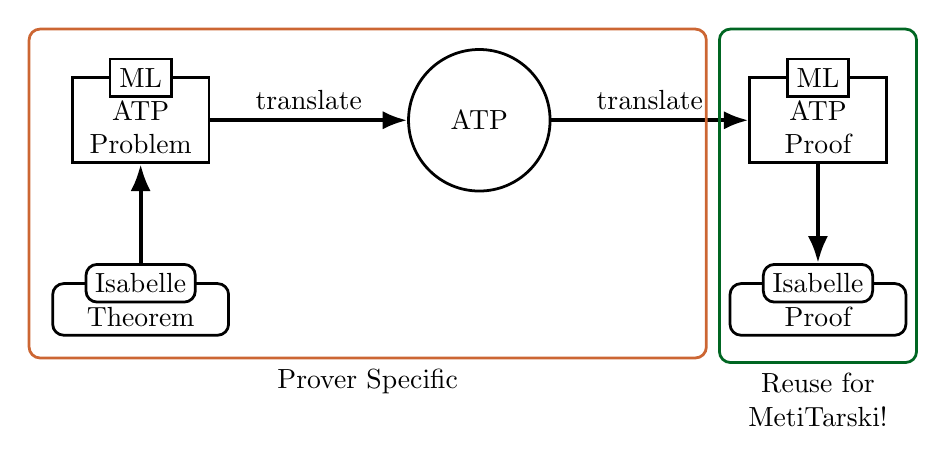
\begin{tikzpicture}
\node (atpProb) [align = center, text width = 1.5cm, draw, line width=1pt] {\\ATP Problem};
\node (atpProbTitle) [fancytitle, above=-0.27cm, line width=1pt] at (atpProb.north) {ML};

\node (isa) [align = center, text width = 2cm, draw, rounded corners, line width=1pt, below=1.5cm of atpProb] {\\Theorem};
\node (isaTitle) [fancytitle, rounded corners, above=-0.27cm, line width=1pt] at (isa.north) {Isabelle};

\node (atp) [circle, align = center, text width = 1.5cm, draw, line width=1pt, right=2.5cm of atpProb] {ATP};

\node (atpProof) [align = center, text width = 1.5cm, draw, line width=1pt, right=2.5cm of atp] {\\ATP Proof};
\node (atpProofTitle) [fancytitle, above=-0.27cm, line width=1pt] at (atpProof.north) {ML};

\node (isaProof) [align = center, text width = 2cm, draw, rounded corners, line width=1pt, below=1.5cm of atpProof] {\\Proof};
\node (isaProofTitle) [fancytitle, rounded corners, above=-0.27cm, line width=1pt] at (isaProof.north) {Isabelle};

\draw[-{Latex},line width=1.5pt, black]
	(isaTitle) edge (atpProb);

\draw[-{Latex},line width=1.3pt, black]
	(atpProb) edge
		node [align = center, text width = 1.5cm, above] {translate} 
	(atp);
	
\draw[-{Latex},line width=1.3pt, black]
	(atp) edge
		node (trans) [align = center, text width = 1.5cm, above] {translate} 
	(atpProof);	

\draw[-{Latex},line width=1.5pt, black]
	(atpProof) edge (isaProofTitle);

\node (box1) [fit={($(isa)+(-1.3cm, -0.5cm)$) ($(trans)-(-0.6cm, 0cm)$) ($(atpProbTitle)+(0cm, 0.5cm)$)}, draw, rounded corners, color=colorThree, line width = 1pt] {};

\node [align = center, text width = 3cm, below=0cm of box1] {Prover Specific};

\node (box2) [fit={(isaProof) ($(isaProofTitle)+(0cm, -0.89cm)$) ($(atpProofTitle)+(0cm, 0.5cm)$)}, draw, rounded corners, color=tikzDarkGreen, line width = 1pt] {};

\node [align = center, text width = 2cm, below=0cm of box2] {Reuse for MetiTarski!};

\end{tikzpicture}
\end{figure}

	\note[item] {When the user invokes Sledgehammer the current goal is translated into some intermediate form, this ATP problem, which is an ML datastructure. This is given to the ATP, it comes up with a proof, which you can put into this standard format of an ATP proof, and then translate it to an Isabelle proof. This is of course a simplified diagram of what happens but you get the idea.}
	\note[item] {The left part of the diagram is specific to every prover, because to get the ATP proof we need some information about how the initial Isabelle lemma was encoded. And this of course depends on each prover. But the right part of the diagram does not depend on the prover. And it is actually the more involved part. So the idea was to somehow reuse this part when reconstructing Metitarski proofs.}

\end{frame}

\begin{frame}
\frametitle{Translations}
	\note[item] {I'm going to focus first on the left side of the diagram before, which involves multiple translations of the problem and the proof. The part I said was prover specific.}
	\note[item] {Because Isabelle is written in SML, any code that wants to interface with it must access the ML internals. So all of the code for this diagram is in SML. So for example there is an internal representation of theorems as an ML datatype and you need to use that to manipulate the statement of theorems.}
	\note[item] {Explain difference between higher-order syntax and first-order using +}
	\note[item] {TPTP format is a standard format that ATPs use and MT also uses. So all the Isabelle names and symbols have to be translated to the tptp symbols.}
	\note[item] {The}

\begin{figure}
\scalebox{0.4}{
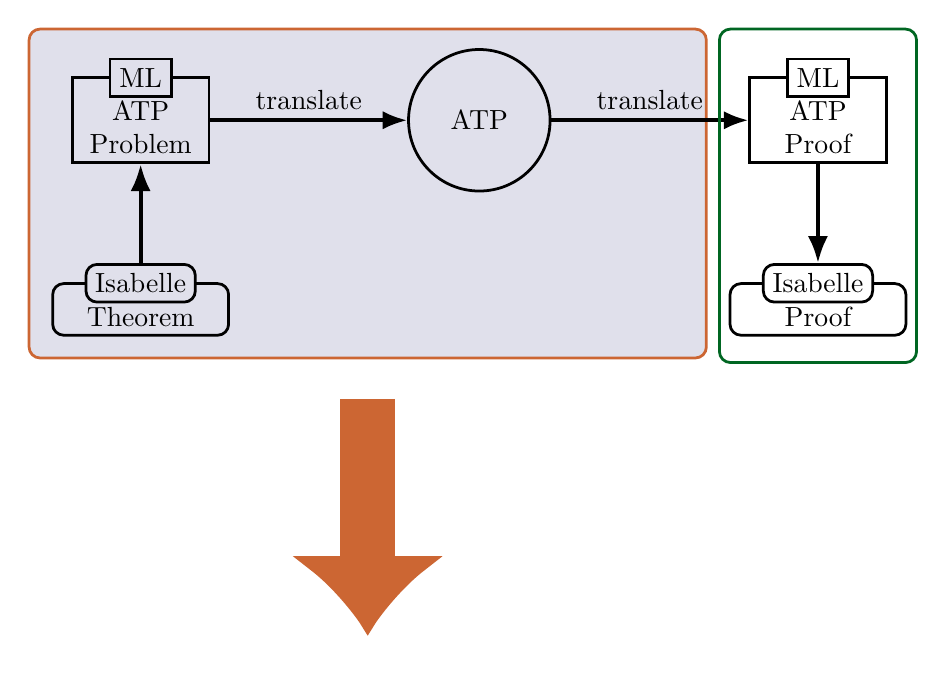
\begin{tikzpicture}
\node (atpProb) [align = center, text width = 1.5cm, draw, line width=1pt] {\textcolor{black}{\\ATP Problem}};
\node (atpProbTitle) [fancytitle, above=-0.27cm, line width=1pt, fill=tikzBack] at (atpProb.north) {ML};

\node (isa) [align = center, text width = 2cm, draw, rounded corners, line width=1pt, below=1.5cm of atpProb] {\\Theorem};
\node (isaTitle) [fancytitle, rounded corners, above=-0.27cm, line width=1pt, fill=tikzBack] at (isa.north) {Isabelle};

\node (atp) [circle, align = center, text width = 1.5cm, draw, line width=1pt, right=2.5cm of atpProb] {ATP};

\node (atpProof) [align = center, text width = 1.5cm, draw, line width=1pt, right=2.5cm of atp] {\\ATP Proof};
\node (atpProofTitle) [fancytitle, above=-0.27cm, line width=1pt] at (atpProof.north) {ML};

\node (isaProof) [align = center, text width = 2cm, draw, rounded corners, line width=1pt, below=1.5cm of atpProof] {\\Proof};
\node (isaProofTitle) [fancytitle, rounded corners, above=-0.27cm, line width=1pt] at (isaProof.north) {Isabelle};

\draw[-{Latex},line width=1.5pt, black]
	(isaTitle) edge (atpProb);

\draw[-{Latex},line width=1.3pt, black]
	(atpProb) edge
		node [align = center, text width = 1.5cm, above] {translate} 
	(atp);
	
\draw[-{Latex},line width=1.3pt, black]
	(atp) edge
		node (trans) [align = center, text width = 1.5cm, above] {translate} 
	(atpProof);	

\draw[-{Latex},line width=1.5pt, black]
	(atpProof) edge (isaProofTitle);

\begin{scope}[on background layer]
\node (box1) [fit={($(isa)+(-1.3cm, -0.5cm)$) ($(trans)-(-0.6cm, 0cm)$) ($(atpProbTitle)+(0cm, 0.5cm)$)}, draw, rounded corners, color=colorThree, line width = 1pt, fill=tikzBack] {};
\end{scope}

%\node [align = center, text width = 3cm, below=0cm of box1] {Prover Specific};

\node (box2) [fit={(isaProof) ($(isaProofTitle)+(0cm, -0.89cm)$) ($(atpProofTitle)+(0cm, 0.5cm)$)}, draw, rounded corners, color=tikzDarkGreen, line width = 1pt] {};

%\node [align = center, text width = 2cm, below=0cm of box2] {Reuse for MetiTarski!};

%arrow
\draw[-{Latex[width=2cm, length=1cm]},line width=20pt, colorThree]
	($(box1.south)+(0, -0.5cm)$) -- ++(0, -3cm);

\end{tikzpicture}
}

\scalebox{0.7}{
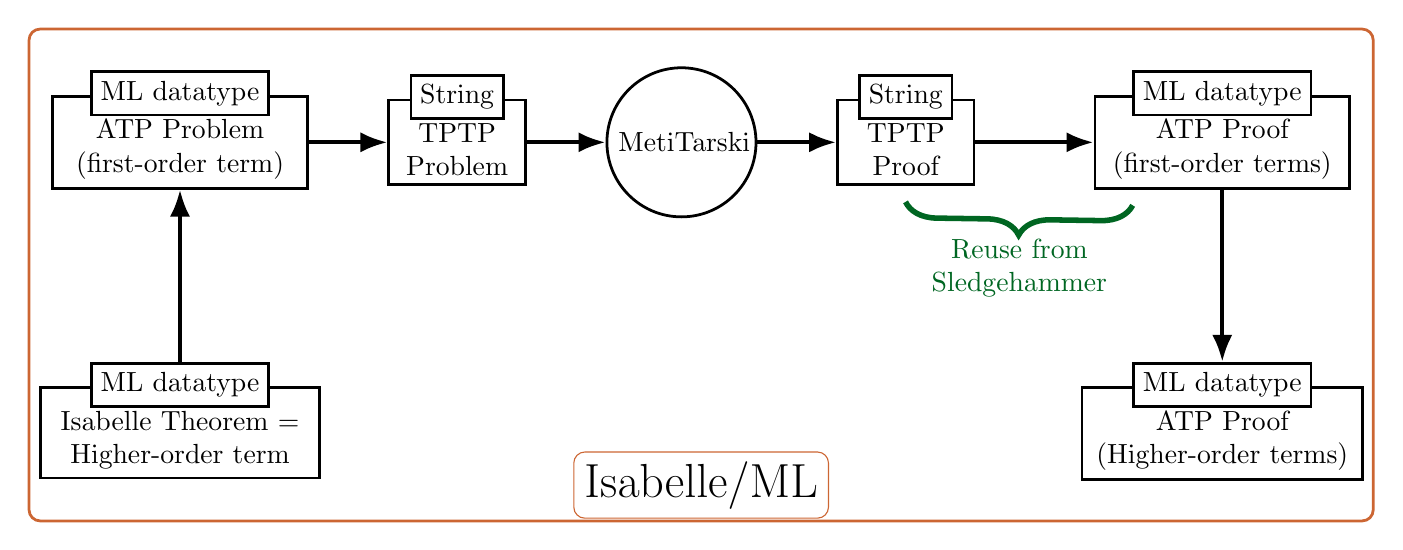
\begin{tikzpicture}
\node (atpProb) [align = center, text width = 3cm, draw, line width=1pt] {\\ATP Problem (first-order term)};
\node (atpProbTitle) [fancytitle, above=-0.27cm, line width=1pt] at (atpProb.north) {ML datatype};

\node (isa) [align = center, text width = 3.3cm, draw, line width=1pt, below=2.5cm of atpProb] {\\Isabelle Theorem = \\ Higher-order term};
\node (isaTitle) [fancytitle, above=-0.27cm, line width=1pt] at (isa.north) {ML datatype};

\node (tptpProb) [align = center, text width = 1.5cm, draw, line width=1pt, right= of atpProb] {\\TPTP Problem};
\node (tptpProbTitle) [fancytitle, above=-0.27cm, line width=1pt] at (tptpProb.north) {String};

\node (atp) [circle, align = center, text width = 1.6cm, draw, line width=1pt, right=1cm of tptpProb] {MetiTarski};

\node (tptpProof) [align = center, text width = 1.5cm, draw, line width=1pt, right=1cm of atp] {\\TPTP Proof};
\node (tptpProofTitle) [fancytitle, above=-0.27cm, line width=1pt] at (tptpProof.north) {String};

\node (atpProof) [align = center, text width = 3cm, draw, line width=1pt, right=1.5cm of tptpProof] {\\ATP Proof (first-order terms)};
\node (atpProofTitle) [fancytitle, above=-0.27cm, line width=1pt] at (atpProof.north) {ML datatype};

\node (atpProofTerm) [align = center, text width = 3.33cm, draw, line width=1pt, below=2.5cm of atpProof] {\\ATP Proof\\ (Higher-order terms)};
\node (atpProofTermTitle) [fancytitle, above=-0.27cm, line width=1pt] at (atpProofTerm.north) {ML datatype};

\draw[-{Latex},line width=1.5pt, black]
	(isaTitle) edge (atpProb);
	
\draw[-{Latex},line width=1.5pt, black]
	(atpProb) edge (tptpProb);
	
\draw[-{Latex},line width=1.5pt, black]
	(tptpProb) edge (atp);
	
\draw[-{Latex},line width=1.5pt, black]
	(atp) edge (tptpProof);
	
\draw[-{Latex},line width=1.5pt, black]
	(tptpProof) edge (atpProof);
	
\draw[-{Latex},line width=1.5pt, black]
	(atpProof) edge (atpProofTermTitle);
	
%brace
\draw[decoration={brace,raise=0.2cm, amplitude=0.4cm, mirror},decorate, line width = 2pt, color=tikzDarkGreen]
	  (tptpProof.south) -- 
	  	node[align = center, below=0.5cm, text width=2.5cm] {Reuse from Sledgehammer} 
	  ($(atpProof.south west)+(0.5cm, 0cm)$);						
	  
\node (box1) [fit={($(isa)+(-1.8cm, -1cm)$) ($(atpProbTitle)+(0cm, 0.7cm)$) (atpProofTerm)}, draw, rounded corners, color=colorThree, line width = 1pt] {};

\node [align = center, text width = 3cm, below=-0.9cm of box1, draw, rounded corners, color = colorThree] 
	{\textcolor{black}{\LARGE Isabelle/ML}};	  
\end{tikzpicture}
}	
\end{figure}	
	
\end{frame}

\begin{frame}
\frametitle{Generating Isabelle Proofs}
	\note[item] {This is the part of Sledgehammer we decided to reuse, the right of the diagram. From the ATP proof with higher-order terms to the actual Isabelle proof text. Sledgehammer already has a lot of sophisticated functionality implemented for this, apart from the textual translation. Explain each of it.}
%	\note[item] {It takes the termified ATP proof with higher-order-terms and translates it to this:}

	\note[item] {But what is difficult is choosing the appropriate proof method for each step in the proof. Because this depends on what steps the prover made. So I had to change the Sledgehammer code to for the MT proofs to work.}
	\note[item] {In particular MetiTarski does some algebraic simplifications so a custom Isabelle method is needed to mirror it. So lately I've been building this method but it still needs more experimentation.}
	\note[item] {I mentioned that MT uses a decision procedure for real closed fields. This needs to be formalised in Isabelle as a proof method. At the moment,one of Larry's students has a formalisation for the univariate case that we can use. But ideally we would extend it to multivariate.}
	\note[item] {In the beginning of the talk I also said that special functions are approximated with polynomials. These approximations are inequalities that MT considers to be axioms. So in Isabelle you would need to prove these inequalities before using them. Some of these have already been formalised but they need to be brought to the exact form that MT uses. While some still need to be proved.}
	
\begin{minipage}{0.45\linewidth}
\begin{figure}
\scalebox{0.4}{
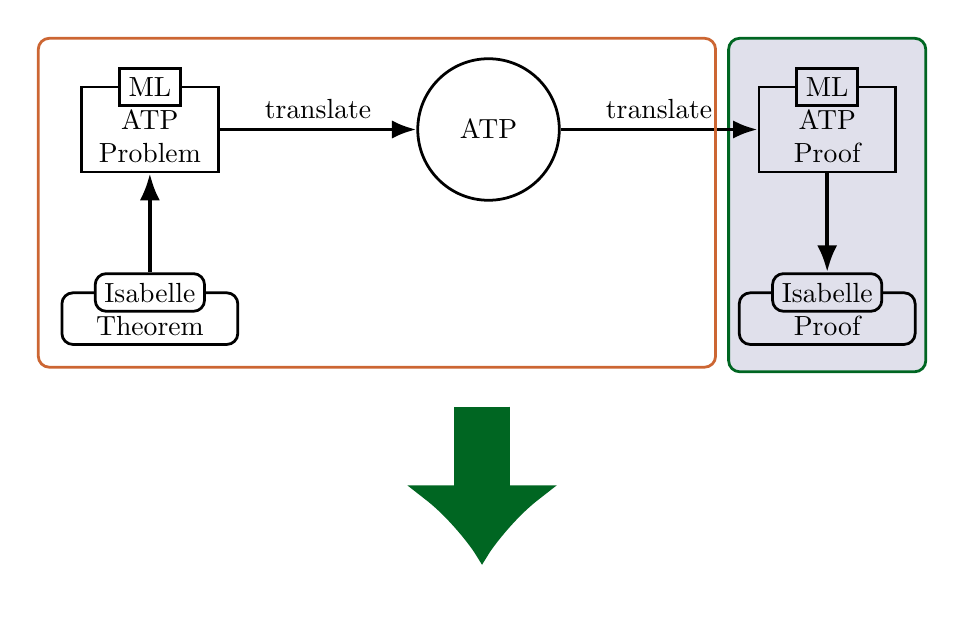
\begin{tikzpicture}
\node (atpProb) [align = center, text width = 1.5cm, draw, line width=1pt] {\textcolor{black}{\\ATP Problem}};
\node (atpProbTitle) [fancytitle, above=-0.27cm, line width=1pt] at (atpProb.north) {ML};

\node (isa) [align = center, text width = 2cm, draw, rounded corners, line width=1pt, below=1.5cm of atpProb] {\\Theorem};
\node (isaTitle) [fancytitle, rounded corners, above=-0.27cm, line width=1pt] at (isa.north) {Isabelle};

\node (atp) [circle, align = center, text width = 1.5cm, draw, line width=1pt, right=2.5cm of atpProb] {ATP};

\node (atpProof) [align = center, text width = 1.5cm, draw, line width=1pt, right=2.5cm of atp] {\\ATP Proof};
\node (atpProofTitle) [fancytitle, above=-0.27cm, line width=1pt, fill=tikzBack] at (atpProof.north) {ML};

\node (isaProof) [align = center, text width = 2cm, draw, rounded corners, line width=1pt, below=1.5cm of atpProof] {\\Proof};
\node (isaProofTitle) [fancytitle, rounded corners, above=-0.27cm, line width=1pt, fill=tikzBack] at (isaProof.north) {Isabelle};

\draw[-{Latex},line width=1.5pt, black]
	(isaTitle) edge (atpProb);

\draw[-{Latex},line width=1.3pt, black]
	(atpProb) edge
		node [align = center, text width = 1.5cm, above] {translate} 
	(atp);
	
\draw[-{Latex},line width=1.3pt, black]
	(atp) edge
		node (trans) [align = center, text width = 1.5cm, above] {translate} 
	(atpProof);	

\draw[-{Latex},line width=1.5pt, black]
	(atpProof) edge (isaProofTitle);


\node (box1) [fit={($(isa)+(-1.3cm, -0.5cm)$) ($(trans)-(-0.6cm, 0cm)$) ($(atpProbTitle)+(0cm, 0.5cm)$)}, draw, rounded corners, color=colorThree, line width = 1pt] {};


%\node [align = center, text width = 3cm, below=0cm of box1] {Prover Specific};

\begin{scope}[on background layer]
\node (box2) [fit={(isaProof) ($(isaProofTitle)+(0cm, -0.89cm)$) ($(atpProofTitle)+(0cm, 0.5cm)$)}, draw, rounded corners, color=tikzDarkGreen, line width = 1pt, fill=tikzBack] {};
\end{scope}

%\node [align = center, text width = 2cm, below=0cm of box2] {Reuse for MetiTarski!};

\node (box) [fit={(box1) (box2)}] {};

%arrow
\draw[-{Latex[width=2cm, length=1cm]},line width=20pt, tikzDarkGreen]
	($(box.south)+(0, -0.3cm)$) -- ++(0, -2cm);

\end{tikzpicture}
}
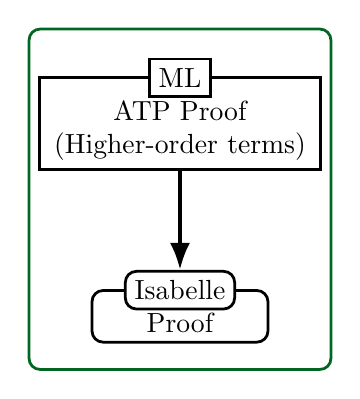
\begin{tikzpicture}
\node (atpProof) [align = center, text width = 3.33cm, draw, line width=1pt] {\\ATP Proof\\(Higher-order terms)};
\node (atpProofTitle) [fancytitle, above=-0.27cm, line width=1pt] at (atpProof.north) {ML};

\node (isaProof) [align = center, text width = 2cm, draw, rounded corners, line width=1pt, below=1.5cm of atpProof] {\\Proof};
\node (isaProofTitle) [fancytitle, rounded corners, above=-0.27cm, line width=1pt] at (isaProof.north) {Isabelle};

\draw[-{Latex},line width=1.5pt, black]
	(atpProof) edge (isaProofTitle);
	
\node (box2) [fit={(isaProof) ($(isaProofTitle)+(0cm, -0.89cm)$) ($(atpProofTitle)+(0cm, 0.5cm)$) (atpProof)}, draw, rounded corners, color=tikzDarkGreen, line width = 1pt] {};	
\end{tikzpicture}
\end{figure}
\end{minipage}	
\hfill
\begin{minipage}{0.45\linewidth}
\only<1>{
Existing functionality:
\vspace{0.2cm}
\begin{itemize}
\setlength\itemsep{1em}
\item Proof redirection;
\item Proof minimization;
\item Proof preplay;
\item Type annotations.
\end{itemize}
}
\only<2>{
MetiTarski requirements:
\vspace{0.2cm}
\begin{itemize}
\setlength\itemsep{1em}
\item Proof methods for:
	\vspace{0.5em}
	\begin{itemize}
	\setlength\itemsep{0.5em}
	\item algebraic simplification;
	\item the decision procedure.
	\end{itemize}
\item Correctness of special function bounds;	
\end{itemize}
}
\end{minipage}
	
\end{frame}

\begin{frame}
\frametitle{What we have so far}
\begin{minipage}{0.35\linewidth}
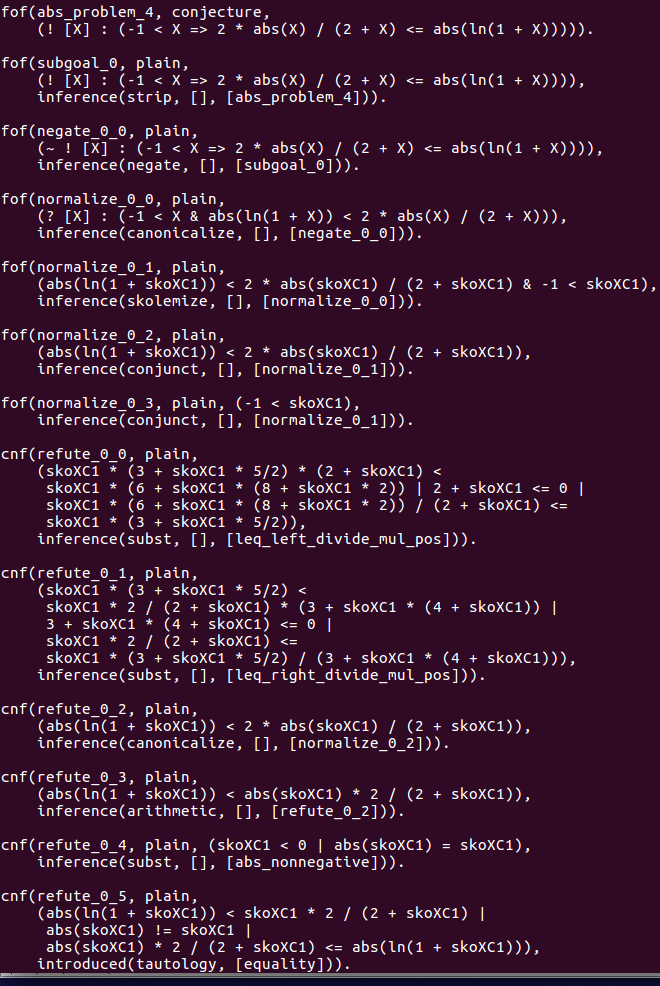
\includegraphics[scale=0.18]{MT_proof}
\end{minipage}
\hfill
\begin{minipage}{0.57\linewidth}
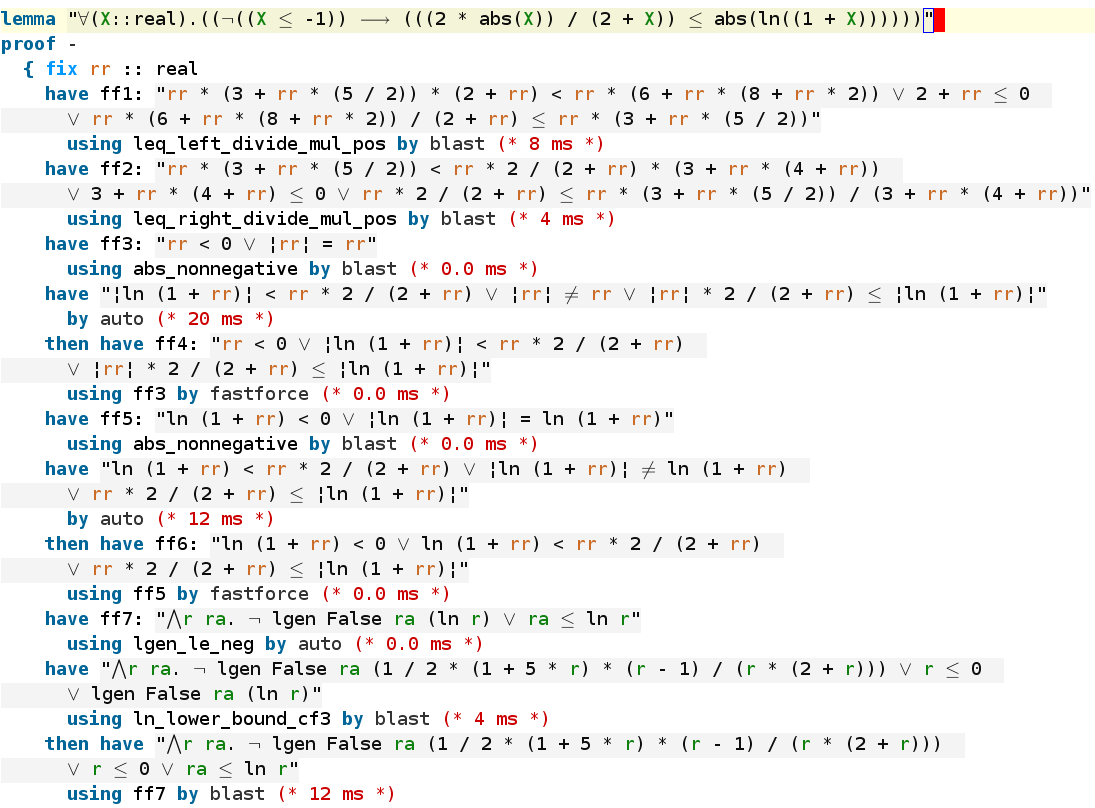
\includegraphics[scale=0.18]{isabelle_proof}
\end{minipage}
\begin{center}
But some proof methods are still missing!
	\note[item] {So this is the same picture as in the beginning. We got the translation that we wanted from a MT proof to an Isabelle proof. But what is missing is appropriate proof methods for some of the steps.}
\end{center}
\end{frame}

\begin{frame}
\frametitle{Summary}

\begin{center}
\begin{minipage}{1\textwidth}
\begin{itemize}
\setlength\itemsep{2em}
\item Translate MetiTarski proofs to Isabelle.
\item Reuse part of the Sledgehammer code.
\item Implement the prover-specific part.
	\note[item] {So we noticed that this tool in Isabelle does something similar for other automitic theorem provers and decided to use part of this functionality. But I had to reimplement the part that was specific to each prover. There is this picture about how Sledgehammer works that I kept showing you.}

\vspace{0.5cm}
\scalebox{0.4}{
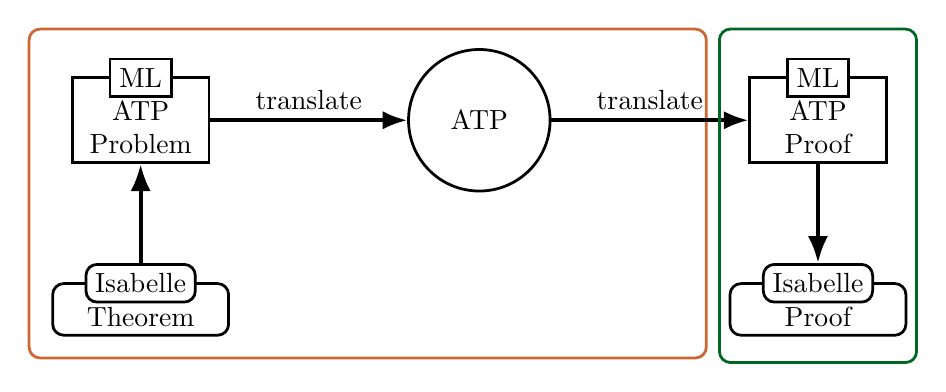
\begin{tikzpicture}
\node (atpProb) [align = center, text width = 1.5cm, draw, line width=1pt] {\textcolor{black}{\\ATP Problem}};
\node (atpProbTitle) [fancytitle, above=-0.27cm, line width=1pt] at (atpProb.north) {ML};

\node (isa) [align = center, text width = 2cm, draw, rounded corners, line width=1pt, below=1.5cm of atpProb] {\\Theorem};
\node (isaTitle) [fancytitle, rounded corners, above=-0.27cm, line width=1pt] at (isa.north) {Isabelle};

\node (atp) [circle, align = center, text width = 1.5cm, draw, line width=1pt, right=2.5cm of atpProb] {ATP};

\node (atpProof) [align = center, text width = 1.5cm, draw, line width=1pt, right=2.5cm of atp] {\\ATP Proof};
\node (atpProofTitle) [fancytitle, above=-0.27cm, line width=1pt] at (atpProof.north) {ML};

\node (isaProof) [align = center, text width = 2cm, draw, rounded corners, line width=1pt, below=1.5cm of atpProof] {\\Proof};
\node (isaProofTitle) [fancytitle, rounded corners, above=-0.27cm, line width=1pt] at (isaProof.north) {Isabelle};

\draw[-{Latex},line width=1.5pt, black]
	(isaTitle) edge (atpProb);

\draw[-{Latex},line width=1.3pt, black]
	(atpProb) edge
		node [align = center, text width = 1.5cm, above] {translate} 
	(atp);
	
\draw[-{Latex},line width=1.3pt, black]
	(atp) edge
		node (trans) [align = center, text width = 1.5cm, above] {translate} 
	(atpProof);	

\draw[-{Latex},line width=1.5pt, black]
	(atpProof) edge (isaProofTitle);

\begin{scope}[on background layer]
\node (box1) [fit={($(isa)+(-1.3cm, -0.5cm)$) ($(trans)-(-0.6cm, 0cm)$) ($(atpProbTitle)+(0cm, 0.5cm)$)}, draw, rounded corners, color=colorThree, line width = 1pt] {};
\end{scope}

%\node [align = center, text width = 3cm, below=0cm of box1] {Prover Specific};

\node (box2) [fit={(isaProof) ($(isaProofTitle)+(0cm, -0.89cm)$) ($(atpProofTitle)+(0cm, 0.5cm)$)}, draw, rounded corners, color=tikzDarkGreen, line width = 1pt] {};
\end{tikzpicture}
}
\vspace{-0.2cm}	
\item Provide appropriate proof methods.
	\note[item] {In the Sldgehammer code I had to customise the code for choosing proof methods. And provide some new proof methods needed in the MT proofs.}
\end{itemize}
\end{minipage}
\end{center}

\end{frame}

\begin{frame}
\frametitle{Still to do}
\begin{itemize}
\setlength\itemsep{2em}
\item Finish proof method for algebraic simplification.
	\note[item] {There is still a certain shape of goals it can't prove}
\item Use the formalisation of the decision procedure.
	\note[item] {At the moment for the steps that require the RCF decision procedure I use a simpler method that is also available in Isabelle and that's easier to use. But this method is less powerful so we wouldn't want to use it in the long-run. But instead we would want to use the formalisation that Wenda has.}
\item Prove more bounds.
	\note[item] {I mentioned that some of the approximations for special functions still need to be proved in Isabelle.}
\item Thoroughly test the proof reconstruction.
	\note[item] {MetiTarski comes with a few hundreds of sample problems and ideally we would like to reconstruct the proofs for all of these in Isabelle. So seeing how many we can do now and where they fail would be a helpful in determining what to focus on next.}			
\end{itemize}
\end{frame}

\end{document}